% Figure: the open-book embedding of the hard universes in R^4 (Theorem~\ref{thm:r4}).
% Requires only tikz. Same colors as the gadget figure: rows vermillion, columns blue.
\begin{figure}[t]
\centering
\providecommand\Description[2][]{}%
\Description{Left: three pages fanning out from a common horizontal binding line that carries three small orange triangles. Right: the three pages drawn flat side by side, each with a blue band (column surface) near the top, blue tubes down to some of the triangles on the binding, dark seals on the band above the others, and a small gray tether.}
\definecolor{obRow}{HTML}{D55E00}%
\definecolor{obCol}{HTML}{0072B2}%
\colorlet{obLine}{obCol!80!black}%
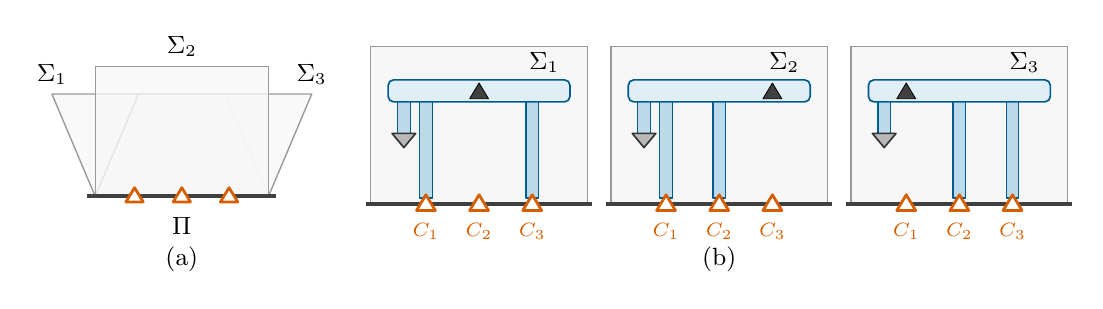
\begin{tikzpicture}[x=1cm,y=1cm,line join=round,
  page/.style={fill=black!3,draw=black!40,line width=0.5pt},
  band/.style={fill=obCol!12,draw=obLine,line width=0.6pt,rounded corners=2pt},
  tube/.style={fill=obCol!26,draw=obLine,line width=0.45pt},
  seal/.style={fill=black!75,draw=black,line width=0.3pt},
  rowtri/.style={fill=white,draw=obRow,line width=1pt},
  teth/.style={fill=black!28,draw=black!80,line width=0.6pt},
  binding/.style={black!75,line width=1.5pt}]
  %%% (a) the book: three pages (half-spaces) with the common boundary Pi
  \begin{scope}[shift={(0,0.1)}]
    \foreach \vx/\vy in {-0.55/1.3,0.55/1.3,0/1.65}
      \path[page,fill opacity=0.8] (0,0) -- (2.2,0) -- (2.2+\vx,\vy) -- (\vx,\vy) -- cycle;
    \node[font=\small,anchor=south] at (-0.55,1.3) {$\Sigma_1$};
    \node[font=\small,anchor=south] at (1.1,1.65) {$\Sigma_2$};
    \node[font=\small,anchor=south] at (2.75,1.3) {$\Sigma_3$};
    \draw[binding] (-0.1,0) -- (2.3,0);
    \foreach \x in {0.5,1.1,1.7} \path[rowtri] (\x-0.11,-0.07) -- (\x+0.11,-0.07) -- (\x,0.11) -- cycle;
    \node[font=\small,anchor=north] at (1.1,-0.14) {$\Pi$};
    \node[font=\small] at (1.1,-0.8) {(a)};
  \end{scope}
  %%% (b) the contents of the three pages, each drawn flat; their bottom edges are the same plane Pi
  % \obpanel{x-offset}{j}{entry row 1}{entry row 2}{entry row 3}
  \def\obpanel#1#2#3#4#5{%
    \begin{scope}[shift={(#1,0)}]
      \path[page] (0,0) rectangle (2.75,2.0);
      \foreach \x/\e in {0.7/#3,1.375/#4,2.05/#5} {\ifnum\e=1 \path[tube] (\x-0.08,0.08) rectangle (\x+0.08,1.31);\fi}
      \path[tube] (0.34,0.9) rectangle (0.5,1.31);
      \path[band] (0.22,1.3) rectangle (2.53,1.58);
      \foreach \x/\e in {0.7/#3,1.375/#4,2.05/#5} {\ifnum\e=0 \path[seal] (\x-0.12,1.34) -- (\x+0.12,1.34) -- (\x,1.54) -- cycle;\fi}
      \path[teth] (0.27,0.9) -- (0.57,0.9) -- (0.42,0.72) -- cycle;
      \node[font=\small] at (2.2,1.8) {$\Sigma_{#2}$};
      \draw[binding] (-0.06,0) -- (2.81,0);
      \foreach \x/\i in {0.7/1,1.375/2,2.05/3} {
        \path[rowtri] (\x-0.12,-0.08) -- (\x+0.12,-0.08) -- (\x,0.12) -- cycle;
        \node[font=\scriptsize,text=obRow,anchor=north] at (\x,-0.12) {$C_{\i}$};
      }
    \end{scope}}
  \obpanel{3.5}{1}{1}{0}{1}
  \obpanel{6.55}{2}{1}{1}{0}
  \obpanel{9.6}{3}{0}{1}{1}
  \node[font=\small] at (7.925,-0.7) {(b)};
\end{tikzpicture}
\caption{The open-book embedding of Theorem~\ref{thm:r4}, an explicit linear version of the pencil-of-$3$-planes embedding of Edelsbrunner and Parsa~\cite{EP14}, drawn schematically for the $3\times3$ matrix~$A$ with columns $(1,0,1)$, $(1,1,0)$, and $(0,1,1)$.
(a)~The row cycles $C_1,C_2,C_3$ lie in the binding plane~$\Pi$, and each column surface $\Sigma_j$ lies in its own page, a closed half of a $3$-dimensional affine subspace of~$\R^4$ bounded by~$\Pi$; distinct pages meet only in~$\Pi$.
(b)~Each page is drawn flat, with its bottom edge representing~$\Pi$.
In the page of~$\Sigma_j$, a tube joins the hole of the socket of position $(i,j)$ to $C_i$ if $A_{ij}=1$, and a seal (black) closes the hole if $A_{ij}=0$; a short tube leads to the private tether~$\Lambda_j$ (gray).
So different surfaces meet only along the row cycles.
Here $P=[3]\times[3]$; in the universe $\cU(P)$, the hole of every socket has both its seal and its tube.}
\label{fig:openbook}
\end{figure}
